\chapter{The Object-Oriented Programming Paradigm}
\label{chap:oopp}
\idx{Object-oriented programming} is a paradigm for encapsulating data and methods into cohesive units. Key features of object-oriented programming are:
\begin{description}
\item[Encapsulation]~\\
Data and methods are collected into a cohesive unit, and an application program need only focus on how to use the object, not on its implementation details.
\item[Inheritance]~\\
Objects are organized in a hierarchy of gradually increased specialty. This promotes a design of code that is of general use, and code reuse.
\item[Polymorphism]~\\
By overriding methods from a base class, derived classes define new data types while their methods still produce results compatible with the base class definitions.
\end{description}

Object-oriented programming has a well-developed methodology for analysis and design. The analysis serves as input to the design phase, where the analysis reveals \idx{what} a program is supposed to do, and the design \idx{how} it is supposed to be doing it. The analysis should be expressed in general terms irrespective of the technologic constraints, while the design should include technological constraints such as defined by the targeted language and hardware.

The primary steps for \idx{object-oriented analysis and design} are:
\begin{enumerate}
\item identify objects,\label{item:analysis}\label{item:identifyObjects}
\item describe object behavior, \label{item:objectBehaviour}
\item describe object interactions, \label{item:objectInteraction}
\item describe some details of the object's inner workings,\label{item:design}\label{item:objectDetails}
\item write a precise description for classes, properties and methods using, e.g., F\#'s XML documentation standard,
\item write mockup code,  \label{item:objectMockup}
\item write unit tests and test the basic framework using the mockup code,\label{item:implementation}
\item replace the mockup with real code while testing to keep track of
  your progress. Extend the unit test as needed,
\item evaluate code in relation to the desired goal,
\item complete your documentation both in-code and outside.
\end{enumerate}
Steps~\ref{item:analysis}--\ref{item:design} are the analysis phase which gradually stops in step~\ref{item:design}, while the design phase gradually starts at step~\ref{item:design} and gradually stops when actual code is written in step~\ref{item:implementation}. Notice that the last steps are identical to imperative programming, \Cref{chap:imperative}. Programming is never a linear experience, and you will often need to go back to previous steps to update or change decisions. You should not refrain from improving your program design and implementation, but you should always be mindful of the goal. Often less than the perfect solution will suffice.

An object-oriented analysis can be a daunting process. A good starting point is a \idx{use case}, \idx{problem statement}, or a \idx{user story}, which in human language describes a number of possibly hypothetical interactions between a user and a system with the purpose of solving some task. Two useful methodologies for performing an object-oriented analysis is the method of nouns-and-verbs and the unified modeling language, described in the following sections.

\section{Identification of Objects, Behaviors, and Interactions by Nouns-and-Verbs}
A key point in object-oriented programming is that objects should to a large extent be independent and reusable. As an example, the type \lstinline|int| models the concept of integer numbers. It can hold integer values from -2,147,483,648 to 2,147,483,647, and a number of standard operations and functions are defined for it. We may use integers in many different programs, and it is certain that the original designers did not foresee our use, but strived to make a general type applicable for many uses. Such a design is a useful goal when designing objects, that is, our objects should model the general concepts and be applicable in future uses. 

Analyzing a specific use-case, good candidates for objects are persons, places, things, events, concept etc., which are almost always characterized by being \idx{nouns} in the text. Interactions between objects are actions that bind objects together, and actions are often associated with \idx{verbs}. When choosing methods, it is important to maintain an object-centered perspective, i.e., for a general-purpose object, we should limit the need for including information about other objects. E.g., a value of type \lstinline|int| need not know anything about the program in which it is being used.

Said briefly, the \idx{nouns-and-verbs method} is:
%
\begin{quote}
  Nouns are object candidates, and verbs are candidate methods that describe interactions between objects.
\end{quote}
%

\section{Class Diagrams in the Unified Modelling Language}
Having found an initial list of candidate objects and interactions, it is often useful to make a drawing of these relations with an increased focus on the object's inner workings. A \idx{class diagram} is a schematic drawing of the program, highlighting its object-oriented structure, and we will use the \idx{Unified Modelling Language 2} (\idx{UML}) \cite{uml2} standard. The standard is very broad, and here we will discuss structure diagrams for use in describing objects. 

A class is drawn as shown in \Cref{fig:class}.
\begin{figure}
  \centering
  \begin{tikzpicture}
    \begin{class}[text width=9cm]{ClassName}{0,0}
      \attribute{value-identifier : type}
      \attribute{value-identifier : type = default value}
      \operation{function-identifier (arg : type) (arg : type) ... : type}
      % virtual operation
      \operation[0]{function-identifier (arg : type) (arg : type) ... : type}
    \end{class}
    \end{tikzpicture}
  \caption{A UML diagram for a class consists of it's name, zero or more attributes, and zero or more methods.}
  \label{fig:class}
\end{figure}
In UML, classes are represented as boxes with their class name. Depending on the desired level of details, zero or more properties and methods are described. These describe the basic interface to the class and objects of its type. Abstract members that require an implementation are shown in cursive. Here we have used F\# syntax to conform with this book theme, but typically C\# syntax is used.
%
\begin{comment}
\begin{figure}
  \centering
  \begin{tikzpicture}%[show background grid] 
    \begin{class}[text width=7cm]{Class}{0,0} \attribute{+ Public}
      \attribute{\# Protected}
      \attribute{- Private}
      \attribute{$\sim$ Package} 
    \end{class}
    \begin{class}[text width=7cm]{BankAccount}{0,-3} \attribute{+ owner : String}
      \attribute{+ balance : Dollars}
      \operation{+ deposit( amount : Dollars )} \operation{+ withdrawal( amount : Dollars )} \operation{\# updateBalance( newBalance : Dollars
        )} 
    \end{class}
  \end{tikzpicture}
  \caption{visibility}
  \label{fig:visibility}
\end{figure}
\begin{figure}
  \centering
  \begin{tikzpicture}
    \begin{abstractclass}[text width=5cm]{BankAccount
      }{0 ,0}
      \attribute{owner : String}
      \attribute{balance : Dollars = 0}
      \operation{deposit(amount : Dollars)} \operation[0]{withdrawl(amount : Dollars)}
    \end{abstractclass} 
  \end{tikzpicture}
  \caption{abstract class}
  \label{fig:abstractClass}
\end{figure}
\end{comment}
%
Interfaces are a special type of class that require an implementation. To highlight this, UML uses the notation shown in \Cref{fig:interface}.\jon{Add programming examples for each of these UML structures}
\begin{figure}
  \centering
  \begin{tikzpicture}%[show background grid] 
    \begin{interface}[text width=9cm]{InterfaceName}{0,0}
      \attribute{value-identifier : type}
      \attribute{value-identifier : type = default value}
      \operation{function-identifier (arg : type) (arg : type) ... : type}
    \end{interface} 
  \end{tikzpicture}
  \caption{An interface is a class that requires an implementation.}
  \label{fig:interface}
\end{figure}

 
Relations between classes and objects are indicated by lines and arrows. The most common ones are summarized in \Cref{fig:arrows}.
\begin{figure}
  \centering
  \fbox{
    \begin{tikzpicture}
      % \draw[umlcd style dashed line] (0,4) --(8,4);
      % \draw[splitline] (0,3) --(8,3);
      \node [left] at (-2,5) {Associate:};
      \node (associateLeft) [left] at (0,5) {HostA};
      \node (associateRight) [right] at (8,5) {HostB};
      \association{associateLeft}{objectsAinB}{0..1}{associateRight}{objectsBinA}{0..*} ;
      
      \node [left] at (-2,4) {\parbox[r]{2.5cm}{\raggedleft Unidirectional associate:}};
      \node (uniAssociateLeft) [left] at (0,4) {Host};
      \node (uniAssociateRight) [right] at (8,4) {Guest};
      \unidirectionalAssociation{uniAssociateLeft}{guestObj}{0..*}{uniAssociateRight};

      \node [left] at (-2,3) {Aggregate:};
      \node (aggregateLeft) [left] at (0,3) {Host};
      \node (aggregateRight) [right] at (8,3) {Guest};
      \aggregation{aggregateLeft}{guestObj}{4}{aggregateRight};
      
      \node [left] at (-2,2) {Compose:};
      \node (composeLeft) [left] at (0,2) {Owner};
      \node (composeRight) [right] at (8,2) {Dependent};
      \composition{composeLeft}{depObj}{1..*}{composeRight};
      
      \node [left] at (-2,1) {Implement:};
      \node (interfaceDerived) [left] at (0,1) {Derived};
      \node (interfaceBase) [right] at (8,1) {Interface};
      \draw[umlcd style implement line] (interfaceBase) -- (interfaceDerived);
      
      \node [left] at (-2,0) {Inherit:};
      \node (inheritDerived) [left] at (0,0) {Derived};
      \node (inheritBase) [right] at (8,0) {Base};
      \draw[umlcd style inherit line] (inheritBase) -- (inheritDerived);
    \end{tikzpicture}
  }
  \caption{Arrows used in class diagrams to show relations between objects.}
  \label{fig:arrows}
\end{figure}
Their meaning will be described in detail in the following. 


\subsection{Associations}
A family of relations is association, aggregation, and composition, and these are distinguished by how they handle the objects they are in relation with. The relation between the three relations is shown in \Cref{fig:associationAggregationCompositionRelation}.
\begin{figure}
  \centering
  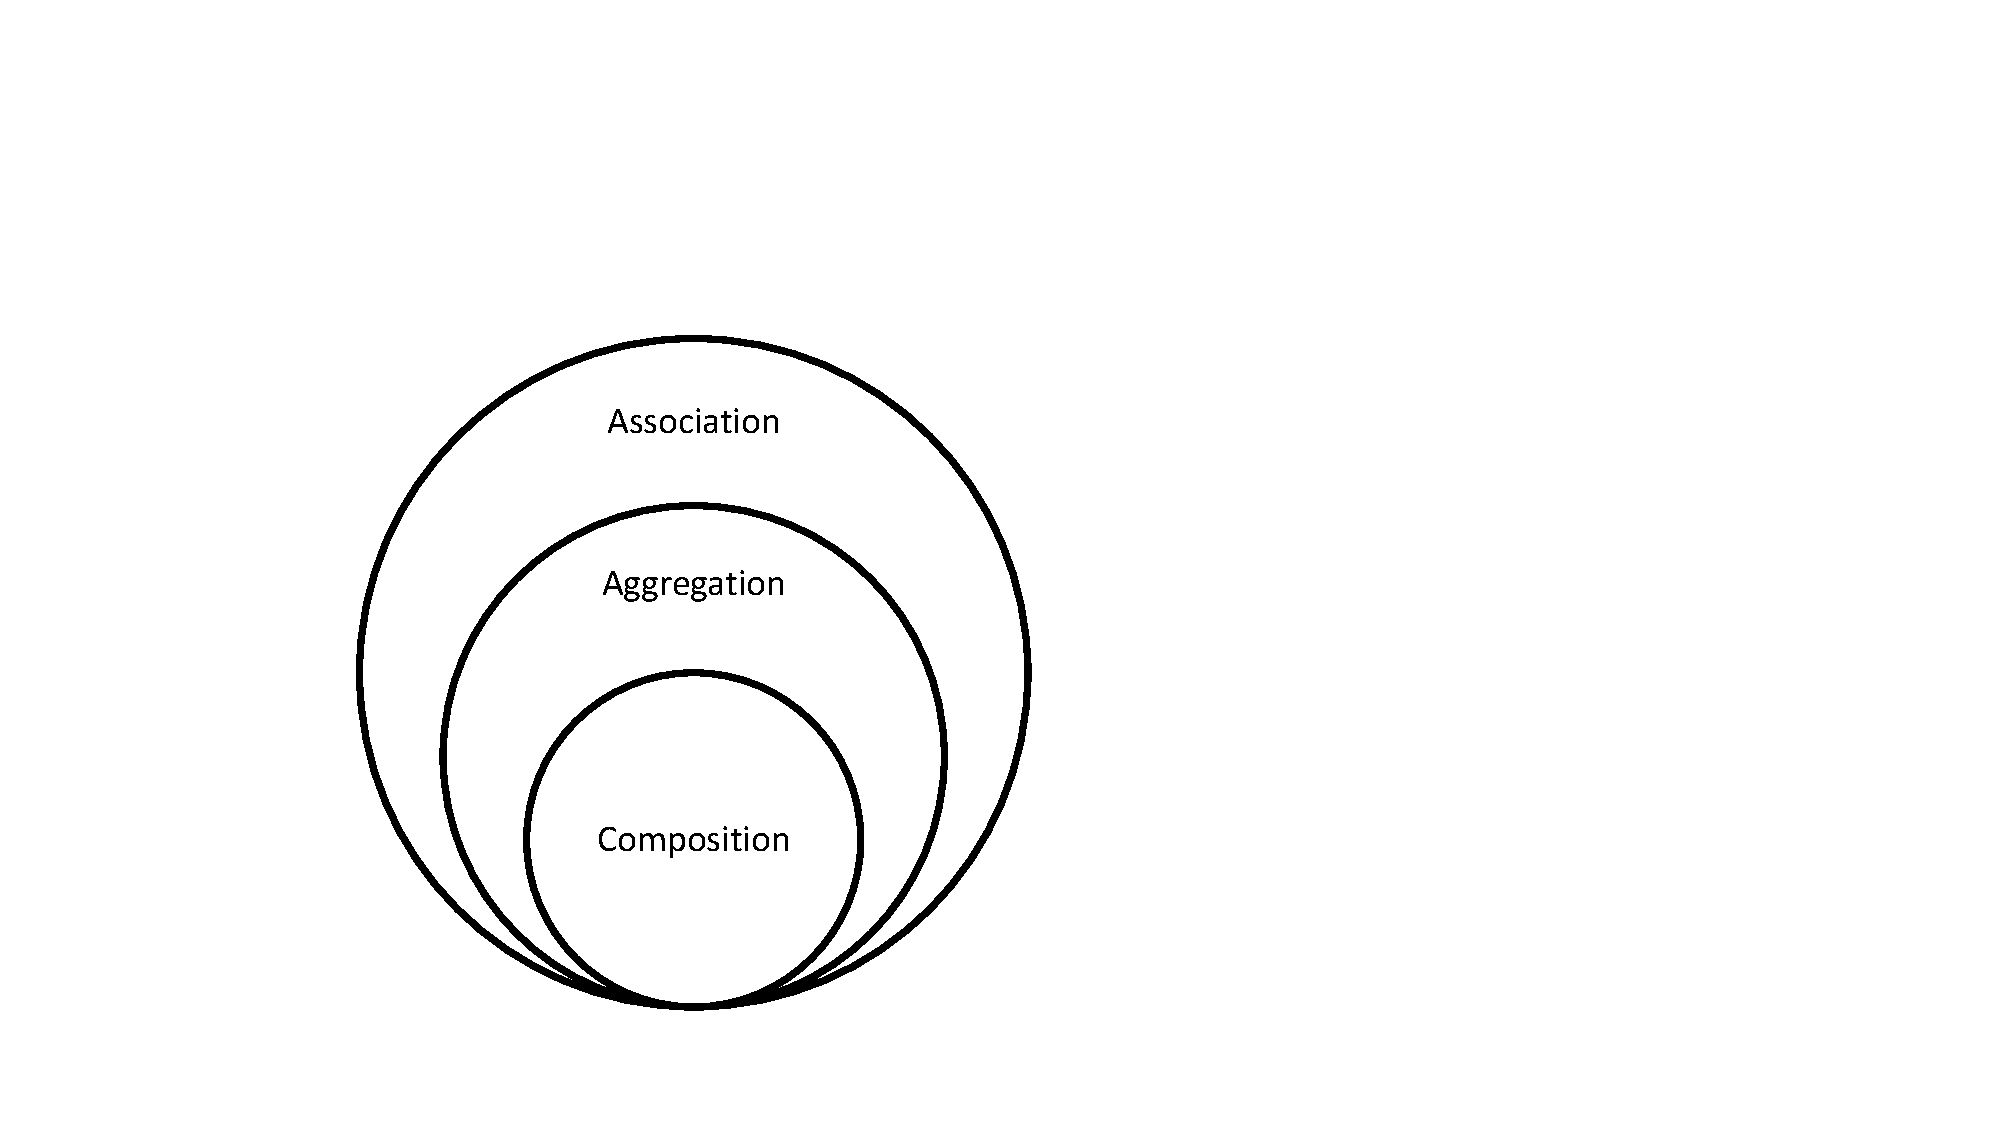
\includegraphics[width=0.45\textwidth]{associationAggregationComposition}
  \caption{The relation between Association, Aggregation and Composition in UML.}
  \label{fig:associationAggregationCompositionRelation}
\end{figure}
Aggregational and compositional are specialized types of associations that imply ownership and are often called \idx[has-a relation]{has-a} relations. A composition is a collection of parts that makes up a whole. In object-oriented design, a compositional relation is a strong relation, where a guest object makes little sense without the host, as a room cannot exist without a house. An aggregation is a collection of assorted items, and in object-oriented design, an aggregational relation is a loose relation, like how a battery can meaningfully be separated from a torchlight. Some associations are neither aggregational nor compositional, and commonly just called an association. An association is a group of people or things linked for some common purpose a cooccurrence. In object-oriented design, associations between objects are the loosest possible relations, like how a student may be associated with the local coffee shop. Sometimes associational relations are called a  \idx[knows-about relation]{knows-about}.

\paragraph{Association}\idxs{association}~\\
The most general type of association, which is just called an association, is the possibility for objects to send messages to each other. This implies that one class knows about the other, e.g., uses it as arguments of a function or similar. A host is associated with a guest if the host has a reference to the guest. Objects are reference types, and therefore, any object which is not created by the host, but where a name is bound to a guest object but not explicitly copied, then this is an association relation.

Bidirectional association means that classes know about each other. The UML notation is shown in \Cref{fig:association}.
\begin{figure}
  \centering
  \begin{tikzpicture}
    \begin{class}{HostA}{0,0}
    \end{class}
    \begin{class}{HostB}{11,0}
    \end{class} 
    \association{HostA}{objectsAinB}{0..1}{HostB}{objectsBinA}{0..*}
  \end{tikzpicture}
  \caption{Bidirectional association is shown as a line with optional annotation.}
  \label{fig:association}
\end{figure}
Association may be annotated by an identifier and a multiplicity. In the figure, HostA has 0 or more variables of type HostB named objectsBinA, while HostB has 0 or 1 variables of HostA named objectsAinB. The multiplicity notation is very similar to F\#'s slicing notation. Typical values are shown in \Cref{tab:multiplicity}.
\begin{table}
  \centering
  \begin{tabular}{|l|l|}
    \hline
    n & exactly n instances\\
    * & zero or more instances \\
    n..m & n to m instances\\
    n..* & from n to infinite instances\\
    \hline
  \end{tabular}
  \caption{Notation for association multiplicities is similar to F\#'s slicing notation.}
  \label{tab:multiplicity}
\end{table}
If the association is unidirectional, then an arrow is added for emphasis, as shown in \Cref{fig:unidirectionalAssociation}.
\begin{figure}
  \centering
  \begin{tikzpicture}
    % \draw[help lines] (-7,-6) grid (6,0);
    \begin{class}{Host}{0,0}
    \end{class}
    \begin{class}{Guest}{9,0}
    \end{class}
    \unidirectionalAssociation{Host}{guestObj}{1}{Guest}
  \end{tikzpicture}  
  \caption{Unidirectional association shows a one-side \emph{has-a} relation.}
  \label{fig:unidirectionalAssociation}
\end{figure}
In this example, Host knows about Guest and has one instance of it, and Guest is oblivious about Host.

A programming example showing a unidirectional association is given in \Cref{umlAssociation}.
% 
\fsCode{umlAssociation}{umlAssociation}{The \lstinline{student} is associated with a \lstinline{teacher}.}{}
% 
Here, the \lstinline{student} is unidirectionally associated with a \lstinline{teacher} since the \lstinline{student} can send and receive messages to and from the \lstinline{teacher}. The \lstinline{teacher}, on the other hand, does not know anything about the \lstinline{student}. In UML this is depicted as shown in \Cref{fig:umlAssociationUML}.
\begin{figure}
  \centering
  \begin{tikzpicture}
    \begin{class}{student}{0,0}
    \end{class}
    \begin{class}{teacher}{9,0}
    \end{class} 
    \unidirectionalAssociation{student}{}{}{teacher}
  \end{tikzpicture}
  \caption{The \lstinline{teacher} and \lstinline{student} objects can access each other's functions, and thus they have an association relation.}
  \label{fig:umlAssociationUML}
\end{figure}

\paragraph{Aggregation}\idxs{aggregation}~\\
Aggregated relationships are a specialization of associations. As an example, an author may have written a book, but once created, the book gets a life independent of the author and may, for example, be given to a reader, and the book continues to exist even when the author dies. That is, In aggregated relations, the host object has a reference to a guest object and may have created the guest, but the guest will be shared with other objects, and when the host is deleted, the guest is not.

Aggregation is illustrated using a diamond tail and an open arrow, as shown in \Cref{fig:aggregation}.
\begin{figure}
  \centering
  \begin{tikzpicture}
    \begin{class}{Host}{0,0}
    \end{class}
    \begin{class}{Guest}{9,0} 
    \end{class}
    \aggregation{Host}{guestObj}{4}{Guest}
  \end{tikzpicture}
  \caption{Aggregation relations are a subset of associations where local aliases are stored for later use.}
  \label{fig:aggregation}
\end{figure}
Here the Host class has stored aliases to four different Guest objects.

An programming example of an aggregation relation is given in \Cref{umlAggregation}.
% 
\fsCode{umlAggregation}{umlAggregation}{The \lstinline{book} has an aggregated relation to \lstinline{author} and \lstinline{reader}.}{}
% 
In aggregated relations, there is a sense of ownership, and in the example, the \lstinline{author} object creates a \lstinline{book} object which is published and bought by a reader. Hence the \lstinline{book} change ownership during the execution of the program. In UML this is to be depicted as shown in \Cref{fig:umlAggregationUML}.
\begin{figure}
  \centering
  \begin{tikzpicture}
    \begin{class}{author}{0,0}
    \end{class}
    \begin{class}{reader}{9,0} 
    \end{class}
    \begin{class}{book}{4.5,2}
    \end{class}
    \aggregation{author}{}{}{book}
    \aggregation{reader}{}{}{book}
  \end{tikzpicture}
  \caption{A book is an object that can be owned by both an author and a reader.}
  \label{fig:umlAggregationUML}
\end{figure}

\paragraph{Composition}\idxs{composition}~\\
A compositional relationship is a specialization of aggregations. As an example, a dog has legs, and dog legs can not very sensibly be given to other animals. That is, in compositional relations, the host creates the guest, and when the host is deleted, so is the guest.  A composition is a stronger relation than aggregation and is illustated using a filled filled diamond tail, as illustrated in \Cref{fig:composition}.
\begin{figure}
  \centering
  \begin{tikzpicture}
    \begin{class}{Owner}{0,0} 
    \end{class}
    \begin{class}{Dependent}{9,0}
    \end{class}
    \composition{Owner}{depObj}{1..*}{Dependent}
  \end{tikzpicture}
  \caption{Composition relations are a subset of aggregation where the host controls the lifetime of the guest objects.}
  \label{fig:composition}
\end{figure}
In this example, Owner has created 1 or more objects of type Dependent, and when Owner is deleted, so are these objects.

A programming example of a composition relation is given in \Cref{umlComposition}.
% 
\fsCode{umlComposition}{umlComposition}{The \lstinline{dog} object is a composition of four \lstinline{leg} objects.}{}
% 
In \Cref{umlComposition}, a \lstinline{dog} object creates four \lstinline{leg} objects, and it makes less sense to be able to turn over the ownership of each \lstinline{leg} to other objects. Thus, a \lstinline{dog} is a composition of \lstinline{leg} objects. Using UML, this should be depicted as shown in \Cref{fig:umlCompositionUML}.
\begin{figure}
  \centering
  \begin{tikzpicture}
    \begin{class}{dog}{0,0} 
    \end{class}
    \begin{class}{leg}{9,0}
    \end{class}
    \composition{dog}{}{}{leg}
  \end{tikzpicture}
  \caption{A dog is a composition of legs.}
  \label{fig:umlCompositionUML}
\end{figure}

\subsection{Inheritance-type relations}
Classes may inherit\idxs{inheritance} other classes where the parent is called the base class and the children its derived classes. Such a relation is often called an \idx[is-a relation]{is-a} relation, since the derived class \emph{is a} kind of base class.

\paragraph{Inheritance}
Inheritance is a relation between properties of classes. As an example, a student and a teacher is a type of person. All persons have names, while a student also has a reading list, and a teacher also has a a set of slides. Thus, both students and teacher may inherit from a person to gain the common property, name. In UML this is illustated with an non-filled, closed arrow as shown in \Cref{fig:inherit}.
\begin{figure}
  \centering
  \begin{tikzpicture}
    \begin{class}[text width=5cm]{BaseClassName}{0,0}
    \end{class}
    \begin{class}[text width=5cm]{DerivedClassA}{-3,-2}
      \inherit{BaseClassName}
    \end{class}
    \begin{class}[text width=5cm]{DerivedClassB}{3,-2} 
      \inherit{BaseClassName} 
    \end{class}
  \end{tikzpicture}
  \caption{Inheritance is shown by a closed arrowhead pointing to the base.}
  \label{fig:inherit}
\end{figure}
Here two classes inherit the base class.

A programming example of an inheritance is given in \Cref{umlInheritance}.
% 
\fsCode{umlInheritance}{umlInheritance}{The \lstinline{student} and the \lstinline{teacher} class inherits from the \lstinline{person} class.}{}
% 
In \Cref{umlInheritance}, the \lstinline{student} and the \lstinline{teacher} classes are derived from the same \lstinline{person} class. Thus, they all three have the \lstinline{name} property. Using UML, this should be depicted as shown in \Cref{fig:umlInheritanceUML}.
\begin{figure}
  \centering
  \begin{tikzpicture}
    \begin{class}{person}{4.5,2}
    \end{class}
    \begin{class}{student}{0,0}
      \inherit{person}
    \end{class}
    \begin{class}{teacher}{9,0} 
      \inherit{person}
    \end{class}
  \end{tikzpicture}
  \caption{A student and a teacher inherit from a person class.}
  \label{fig:umlInheritanceUML}
\end{figure}

\paragraph{Interface}
An interface is a relation between the properties of an abstract class and a regular class. As an example, a television and a car both have buttons, that you can press, although their effect will be quite different. Thus, a television and a car may both implement the same interface. In UML, interfaces are shown similarly to inheritance, but using a stippled line, as shown in \Cref{fig:implement}.
\begin{figure}
  \centering
  \begin{tikzpicture}
    \begin{interface}[text width=5cm]{InterfaceName}{0,0} 
    \end{interface}
    \begin{class}[text width=5cm]{DerivedClassA}{-3,-2}
      \implement{InterfaceName}
    \end{class}
    \begin{class}[text width=5cm]{DerivedClassB}{3,-2} 
      \implement{InterfaceName} 
    \end{class}
  \end{tikzpicture}
  \caption{Implementations of interfaces is shown with stippled line and closed arrowhead pointing to the base.}
  \label{fig:implement}
\end{figure}

A programming example of an interface is given in \Cref{umlInterface}.
% 
\fsCode{umlInterface}{umlInterface}{The \lstinline{television} and the \lstinline{car} class both implement the \lstinline{button} interface.}{}
% 
In \Cref{umlInterface}, the \lstinline{television} and the \lstinline{car} classes implement the \lstinline{button} interface. Hence, although they are different classes, they both have the \lstinline{press ()} method and, e.g., can be given as a function requiring only the existence of the \lstinline{press ()} method. Using UML, this should be depicted as shown in \Cref{fig:umlInterfaceUML}.
\begin{figure}
  \centering
  \begin{tikzpicture}
    \begin{class}{button}{4.5,2}
    \end{class}
    \begin{class}{television}{0,0}
      \implement{button}
    \end{class}
    \begin{class}{car}{9,0} 
      \implement{button}
    \end{class}
  \end{tikzpicture}
  \caption{A student and a teacher inherit from a person class.}
  \label{fig:umlInterfaceUML}
\end{figure}

\subsection{Packages}
\paragraph{Namespace and modules}
For visual flair, modules and namespaces are often visualized as \idx[package]{packages}, as shown in \Cref{fig:package}. A package is like a module in F\#.
\begin{figure}
  \centering
  \begin{tikzpicture} 
    \begin{package}{APackageName}
      \begin{class}[text width=3cm]{Base}{0,0} 
        \attribute{aValue : int = 0}
        \operation{get:  () -> int }
        \operation[0]{set: int -> ()} 
      \end{class}
      \begin{class}[text width=4cm]{Guest}{-4,-4}
        \attribute{aString : string}
        \operation{writeMessage : () -> ()}
      \end{class}
      \begin{class}[text width=6cm]{Derived}{4, -4}
        \inherit{Base} 
        \attribute{dictionary : string list}
        \operation{checkSpelling : string -> bool}
        \operation{set : int -> ()} 
      \end{class}
    \aggregation{Derived}{guestObj}{4}{Guest}
    \end{package} 
  \end{tikzpicture}
  \caption{Packages are a visualizations of modules and namespaces.}
  \label{fig:package}
\end{figure}

\section{Programming Intermezzo: Designing a Racing Game}
An example is the following \idx{problem statement}:
%
\begin{problem}
  Write a racing game, where each player controls his or her vehicle on a track. Each vehicle must have individual features such as top acceleration, speed, and handling. The player must be able to turn the vehicle left and right, and to accelerate up and down. At the beginning of the game, each vehicle is placed behind the starting line. Once the start signal is given, then the players may start to operate their vehicles. The player who first completes 3 rounds wins.
\end{problem}
%
To seek a solution, we will use the \emph{nouns-and-verbs method}. Below, the problem statement is repeated with \noun{nouns} and \vb{verbs} highlighted.
\begin{quote}
  \vb{Write} a \noun{racing game}, where each \noun{player} \vb{controls} his or her \noun{vehicle} on a \noun{track}. Each \noun{vehicle} \vb{must have} individual \noun{features} such as \noun{top acceleration}, \noun{speed}, and \noun{handling}. The \noun{player} \vb{must be} able to \vb{turn} the vehicle left and right, and to \vb{accelerate} up and down. At the \noun{beginning} of the \noun{game}, each \noun{vehicle} \vb{is placed} behind the \noun{starting line}. Once the \noun{start signal} is given, then the \noun{players} \vb{may start} to \vb{operate} their \noun{vehicles}. The \noun{player} who first \vb{completes} 3 \noun{rounds} \vb{wins}.
\end{quote}
The above nouns and verbs are candidates for objects, their behaviour, and their interaction. A deeper analysis is:
\begin{description}
\item[Identification of objects by nouns (Step~\ref{item:identifyObjects}):]~\\
  Identified unique nouns are: \noun{racing game (game)}, \noun{player}, \noun{vehicle}, \noun{track}, \noun{feature}, \noun{top acceleration}, \noun{speed}, \noun{handling}, \noun{beginning}, \noun{starting line}, \noun{start signal}, \noun{rounds}. From this list we seek cohesive units that are independent and reusable. The nouns
  \begin{quote}
    \noun{game}, \noun{player}, \noun{vehicle}, and \noun{track}
  \end{quote}
  seem to fulfill these requirements, while all the rest seems to be features of the former and thus not independent concepts. E.g., \noun{top acceleration} is a feature of a \noun{vehicle}, and \noun{starting line} is a feature of a \noun{track}.
\item[Object behavior and interactions by verbs (Steps~\ref{item:objectBehaviour}  and~\ref{item:objectInteraction}):]~\\
  To continue our object-oriented analysis, we will consider the object candidates identified above, and verbalize how they would act as models of general concepts useful in our game.
\begin{description}
\item[\noun{player}] The \noun{player} is associated with the following verbs:
  \begin{itemize}
  \item A \noun{player} \vb{controls}/\vb{operates} a \noun{vehicle}. 
  \item A \noun{player} \vb{turns} and \vb{accelerates} a \noun{vehicle}.
  \item A \noun{player} \vb{completes} \noun{rounds}. 
  \item A \noun{player} \vb{wins}. 
  \end{itemize}
  Verbalizing a \noun{player}, we say that a \noun{player} in general must be able to control the \noun{vehicle}. In order to do this, the \noun{player} must receive information about the \noun{track} and all \noun{vehicles}, or at least some information about the nearby \noun{vehicles} and \noun{track}. Furthermore, the \noun{player} must receive information about the state of the \noun{game}, i.e., when the race starts and stops.
\item[\noun{vehicle}] A \noun{vehicle} is controlled by a \noun{player} and further associated with the following verbs:
  \begin{itemize}
  \item A \noun{vehicle} \vb{has} \noun{features} \noun{top acceleration}, \noun{speed}, and \noun{handling}. 
  \item A \noun{vehicle} \vb{is placed} on the \noun{track}.
  \end{itemize}
  To further describe a \noun{vehicle}, we say that a \noun{vehicle} is a model of a physical object which moves around on the \noun{track} under the influence of a \noun{player}. A \noun{vehicle} must have a number of attributes such as top acceleration, speed, and handling, and must be able to receive information about when to turn and accelerate. A \noun{vehicle} must be able to determine its location in particular if it is on or off \noun{track} and, and it must be able to determine if it has crashed into an obstacle such as another \noun{vehicle}.
\item[\noun{track}] A \noun{track} is the place where vehicles operate and is further associated with the following verbs:
  \begin{itemize}
  \item A \noun{track} \vb{has} a \noun{starting line}.
  \item A \noun{track} \vb{has} \vb{rounds}.
  \end{itemize}
  Thus, a \noun{track} is a fixed entity on which the \noun{vehicles} race. It has a size and a shape, a starting and a finishing line, which may be the same, and \noun{vehicles} may be placed on the \noun{track} and can move on and possibly off the \noun{track}.
\item[\noun{game}] Finally, a \noun{game} is associated with the following verbs:
  \begin{itemize}
  \item A \noun{game} \vb{has} a \noun{beginning} and a \noun{start signal}. 
  \item A \noun{game} \vb{can be} \noun{won}.
  \end{itemize}
  A \noun{game} is the total sum of all the \noun{players}, the \noun{vehicles}, the \noun{tracks}, and their interactions. A \noun{game} controls events, including inviting \noun{players} to race, sending the \noun{start signal}, and monitoring when a \noun{game} is finished and who \noun{won}.
\end{description}
From the above we see that the object candidates \noun{features} seems to be a natural part of the description of the \noun{vehicle}'s attributes, and similarly, a \noun{starting line} may be an intricate part of a \noun{track}. Also, many of the \idx{verbs} used in the problem statement and in our extended verbalization of the general concepts indicate methods that are used to interact with the object. The object-centered perspective tells us that for a general-purpose \noun{vehicle} object, we need not include information about the \noun{player}, analogous to how a value of type \lstinline|int| need not know anything about the program, in which it is being used. In contrast, the candidate \noun{game} is not as easily dismissed and could be used as a class which contains all the above.

With this description, we see that 'start signal' can be included as a natural part of the game object. Being confident in our working hypothesis of the essential objects for the solution, we continue our investigation into further details about the objects and their interactions.

\item[Analysis details (Step~\ref{item:objectDetails}):]~\\
  A class diagram of our design for the proposed classes and their relations is shown in \Cref{fig:race}.
\begin{figure}
  \centering
  \begin{tikzpicture} 
    \begin{package}{Race}
      \begin{class}[text width=6cm]{Game}{-4,0} 
        \attribute{// Racing clock}
        \attribute{time : int = 0}
        \operation{// Setup game}
        \operation{// m human and n computer}
        \operation{// players}
        \operation{initialize:  (m : int) (n : int) -> ()}
        \operation{// Main loop, starts race and time,}
        \operation{// finishes when winner found or}
        \operation{// no players left. In each iteration,}
        \operation{// clock is forwarded, each player}
        \operation{// is queried for their action,}
        \operation{// vehicles are updated, crashes}
        \operation{// are checked and handled,}
        \operation{// finish conditions are checked. }
        \operation{race:  () -> () }
      \end{class}
      \begin{class}[text width=6.5cm]{Vehicle}{4.5,0} 
        \attribute{// size as a circle}
        \attribute{size : int}
        \attribute{// Present coordinate}
        \attribute{position : (int * int) option = None}
        \attribute{// Present acceleration vector}
        \attribute{acceleration : int * int = (0, 0)}
        \attribute{// Present speed vector}
        \attribute{velocity : int * int = (0, 0)}
        \attribute{// Handling ability 0.0..1.0, 1.0 is best}
        \attribute{handling : float = 0}
        \operation{// Change acceleration by argument}
        \operation{accelerate :  int * int -> () }
        \operation{// Update position after a clock tick}
        \operation{update :  () -> () }
        \operation{// Perform crash action}
        \operation{crash :  () -> () }
      \end{class}
      \begin{class}[text width=6cm]{Player}{4.5,-12.1} 
        \attribute{// Number of rounds remaining}
        \attribute{roundsLeft : int option = None}
        \attribute{// Human or computer player}
        \attribute{human : bool = true}
        \operation{// Query user for acceleration}
        \operation{getAction:  () -> (int * int) option}
      \end{class}
      \begin{class}[text width=6cm]{Track}{-4,-11}
        \attribute{// A curve as by a list of}
        \attribute{// coordinates}
        \attribute{shape : (int * int) list}
        \attribute{// Constant width of curve}
        \attribute{width : int}
        \attribute{// Index into shape list}
        \attribute{startLine : int}
        \attribute{// Index into shape list}
        \attribute{finishLine : int}
        \operation{// Is a position is on or off track}
        \operation{onTrack: int * int -> bool}
      \end{class}
      \composition{Game}{player}{1..(m+n)}{Player}
      \composition{Game}{track}{1}{Track}
      \composition{Game}{vehicle}{m+n}{Vehicle}
      \aggregation{Player}{vehicle}{m+n}{Vehicle}
      \aggregation{Player}{track}{1}{Track}
      %\aggregation{Vehicle}{track}{1}{Track}
    \end{package}
  \end{tikzpicture}
  \caption{A class diagram for a racing game.}
  \label{fig:race}
\end{figure}
\end{description}
In the present description, there will be a single Game object that initializes the other objects, executes a loop updating the clock, queries the players for actions, and informs the vehicles that they should move and under what circumstances. The track has been chosen to be dumb and does not participate much in the action. Player's method getAction will be an input from a user by keyboard, joystick or similar, but the complexity of the code for a computer player will be large, since it needs to take a sensible decision based on the track and the location of the other vehicles. What at present is less clear, is whether it is the responsibility of Game or Vehicle to detect an off track or a crash event. If a vehicle is to do this, then each vehicle must have aggregated association to all other vehicles and obstacles. So, on the one hand, it would seem an elegant delegation of responsibilities that a vehicle knows whether it has crashed into an obstacle or not, but on the other hand, it seems wasteful of memory resources to have duplicated references of all obstacles in every vehicle. The final choice is thus one of elegance versus resource management, and in the above, we have favored resource management. Thus, the main loop in Game must check all vehicles for a crash event after the vehicle's positions have been updated, and in case of a crash, informs the relevant vehicles.

Having created a design for a racing game, we are now ready to start coding (Step~\ref{item:objectMockup}--). It is not uncommon that transforming our design into code will reveal new structures and problems that possibly require our design to be updated. Nevertheless, a good design phase is almost always a sure course to avoid many problems once coding, since the design phase allows the programmer to think about the problem from a helicopter perspective before tackling details of specific sub-problems.

%%% Local Variables:
%%% TeX-master: "fsharpNotes"
%%% End:

